\documentclass[11pt]{article}
\usepackage{hyperref}
\usepackage{multicol}
\usepackage{multirow}
\usepackage{graphicx}
\usepackage{comment}

\title{\textbf{Superpositions with  \\ Sparse Distributed Memories, High Dimensional and Dense Vectors}} %(and Classification)}}
\author{JW}
\date{}
\begin{document}

\maketitle
\begin{abstract}
Vector representations are standard for representing data.
Aside of the intrisic quality of the vectors, various questions 
arise as they are used in interplay with other data elements,
algorithms and systems.


For three frameworks, 
we focus here on the superposition operation and present a technical review of the observed behaviours. 



%Kanerva's cognitive system naturally expands on much larger and sparser binary vectors. We find that while preserving the computing features of the standard HD architectures, this allows to reduce memory requirements,  
%potentially increasing speed.

%We discuss the cognitive symbolic architecture and its properties within this framework
% and test our proposed alternative against simple alternatives on simple experiments.

\end{abstract}

\section{Introduction}
For modelling and representing data, various attempts have been made
and vector models have been considered for instance with
 vector symbolic architectures or to model data learned from algorithms like neural networks.


One standard way to represent data and even language has became
the standard, dense vectors, a number of floats within a range.

Alternative representations are based on the ideas of Hyperdimensional or high dimensional (HD) computing, which are binary vectors of large size. As an interesting variation, we consider here also a sparse version of these: sparse distributed memories (SDM).
The above framework are introduced in \cite{kanerva1} 
and  \cite{kanerva2} respectively.



\subsection{Operation with vector representations}

We focus here mainly on simple, standard operations on vectors:
\begin{itemize}
\item similarity: an operation measuring similarity between two vectors $sim(\vec v_1,\, \vec v_2)$, e.g. cosine similarity for dense vectors.
\item superposition: given a set of vectors $S=(\vec v_1,\, v_2,\, \dots)$, the operation of adding an additional vector to the set above.
\item proning: the possibility to identify the presence of a sub constituent using similarities. This is achieved by setting thresholds or selecting the most similar elements.
\end{itemize}
Notice that HD and SDM computing allow for a vector symbolic architecture framework, with the design of sets, records and sequences (Kanerva cognitive code \cite{kanerva1}) with properties that are naturally inherited by SDM's.






\section{Experiments with set and random vectors}
Below, for the three vector formalisms, we  produce visualisations of sets robustness under superposition.
The experiment consists in building sets by the superposition of 1 to N random elements.

As a baseline, we start to evaluate the averaged similarity for random vectors.  Then we compare the superposition with N elements to the one with N+1. Finally, we compare the initial random vector with the various  superpositions.

\subsection{Similarities and Superpositions}
The code is available online \footnote{\url{github}}.
\subsubsection{Dense Vectors}
	$superpose_{Dense}(\vec v_1,\, \vec v_2, \, \dots) \to \| \vec v_1 + \vec v_2 \|,$
	whereas $\| \dots \|$ is a normalisation to vector of length 1. \\
	Similarity is the standard cosine similarity.
\subsubsection{HD Computing}
	$superpose_{HD\,\, C.}(\vec v_1,\, \vec v_2, \, \dots) = [ f_{HD}(\vec v_1[1], \, \vec v_2[1], \, \dots), \, \dots, \, f_{HD}(\vec v_1[N], \, \vec v_2[N], \, \dots)],$
	with $f_{HD}(x_1, x_2,\, \dots, \, x_n) = round_{HD}(\sum_i^n x_i/ n) ,$
	$round_{HD} (x)$ is randomized toward $\{0, \, 1 \}$ when $x=0.5$.\\
	Similarity is based on the XOR operation between bits at the same position, which gives the Hamming distance after normalisation $d_{H}(A, B) = (\vec A\,\, XOR\,\, \vec B) / length(\vec A)$.
	We set $similarity(A, B) = 1 - 2*d_H(A, B)$.
		
	
\subsubsection{SDM}
	$superpose_{SDM}(\vec v_1,\, \vec v_2, \, \dots) = Set(Indices(\vec v_1) + Indices(\vec v_2) + \dots), $ indices that allows to characterise SDM. Similarity is as for HD computing, however, in practice, one uses sparse frameworks.

\begin{figure}[h!]
 \begin{center}$
  \begin{array}{cc}
   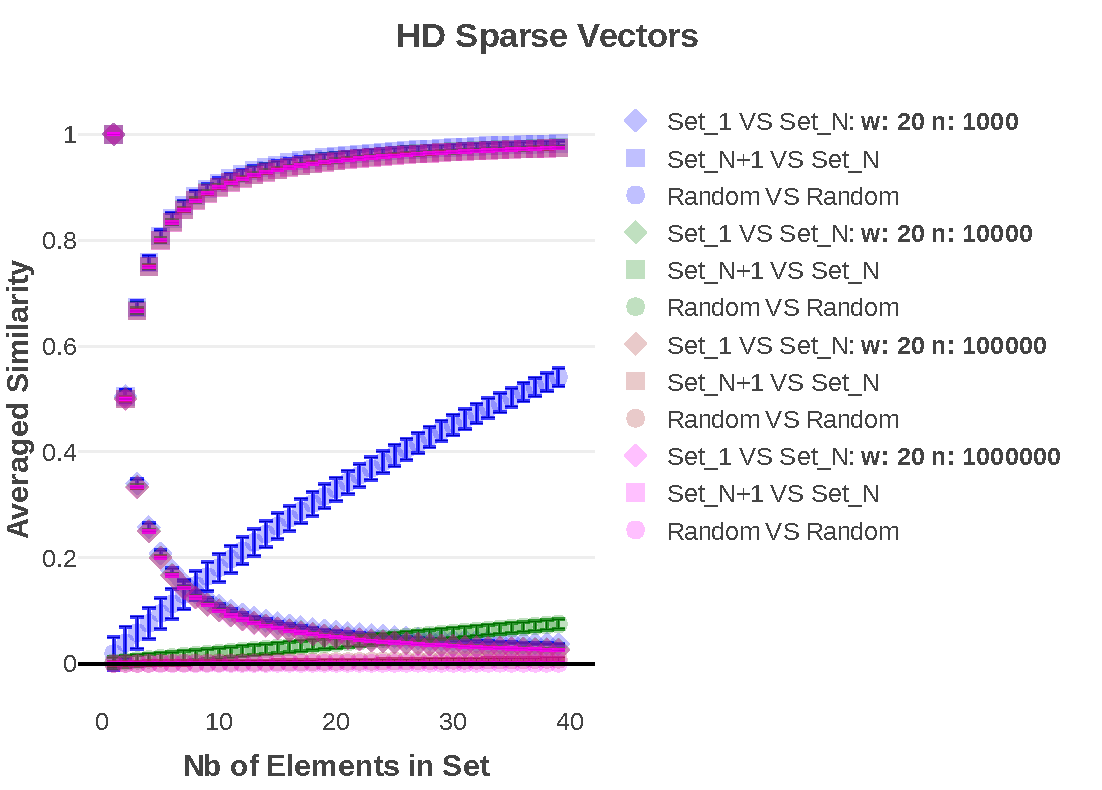
\includegraphics[width=70mm,height=40mm]{../Results/HDSparseFig1Overview.pdf}&
   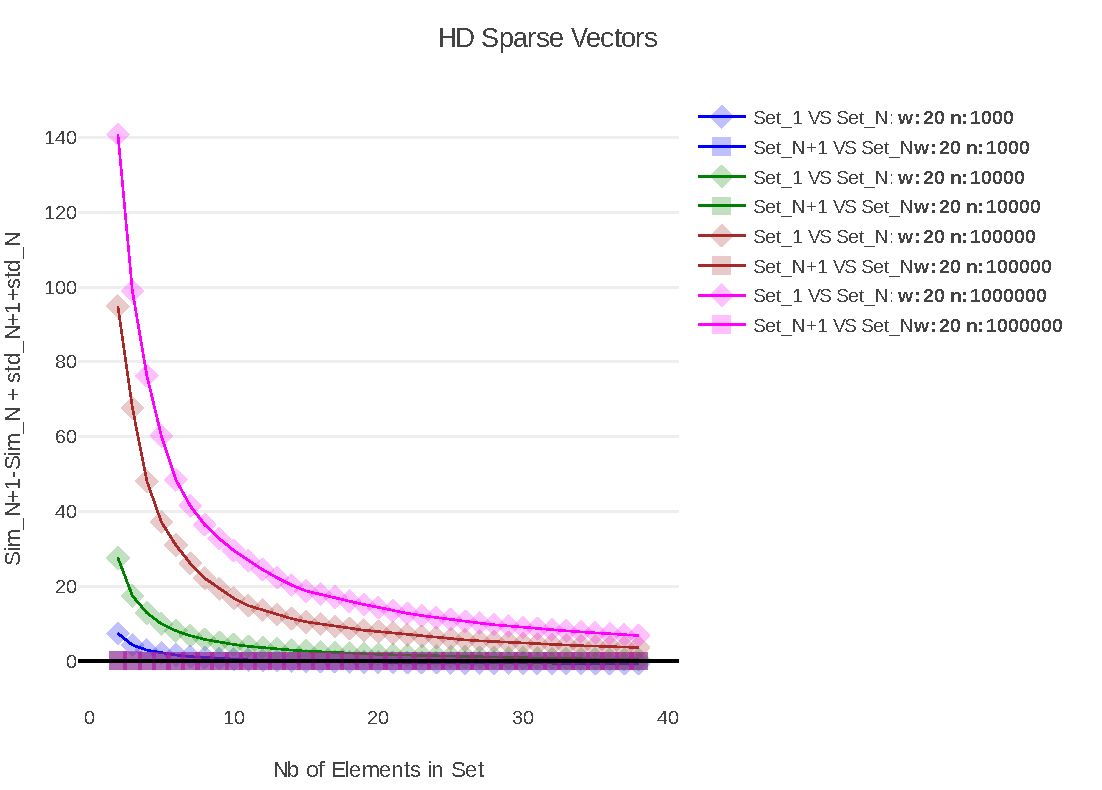
\includegraphics[width=70mm,height=40mm]{../Results/HDSparseFig1Deltas.pdf} \\
   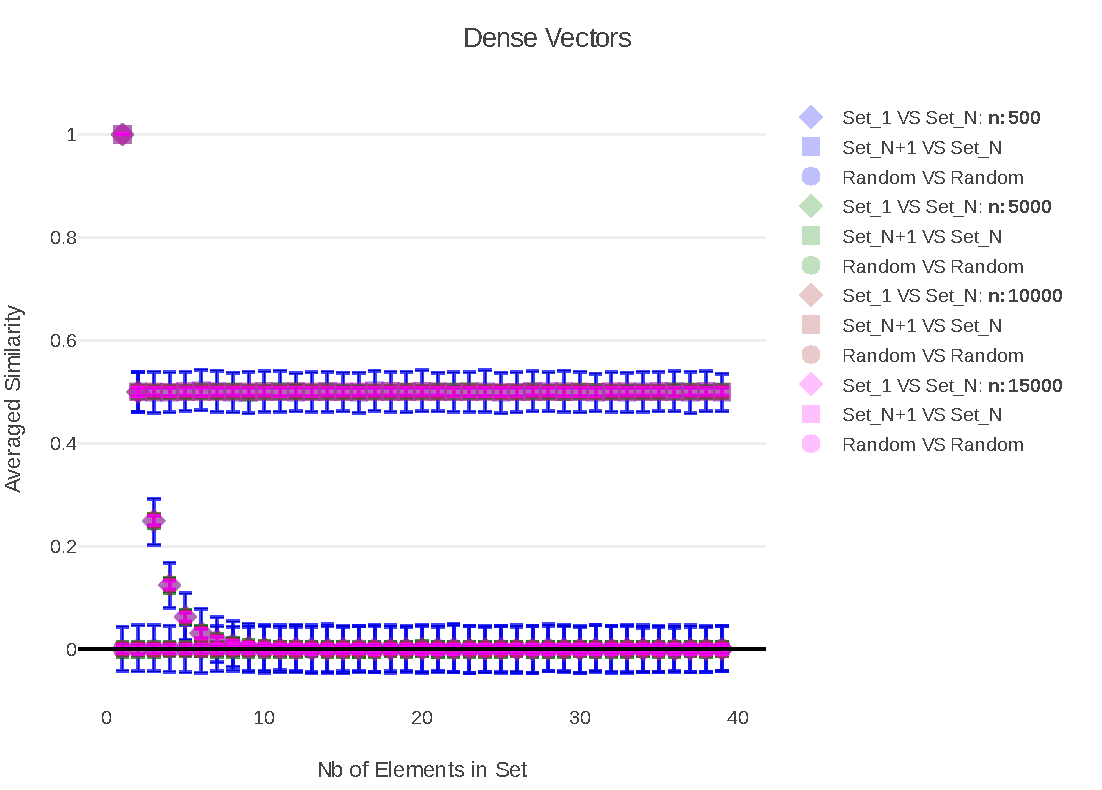
\includegraphics[width=70mm,height=40mm]{../Results/HDBinaryFig1Overview.pdf}&
   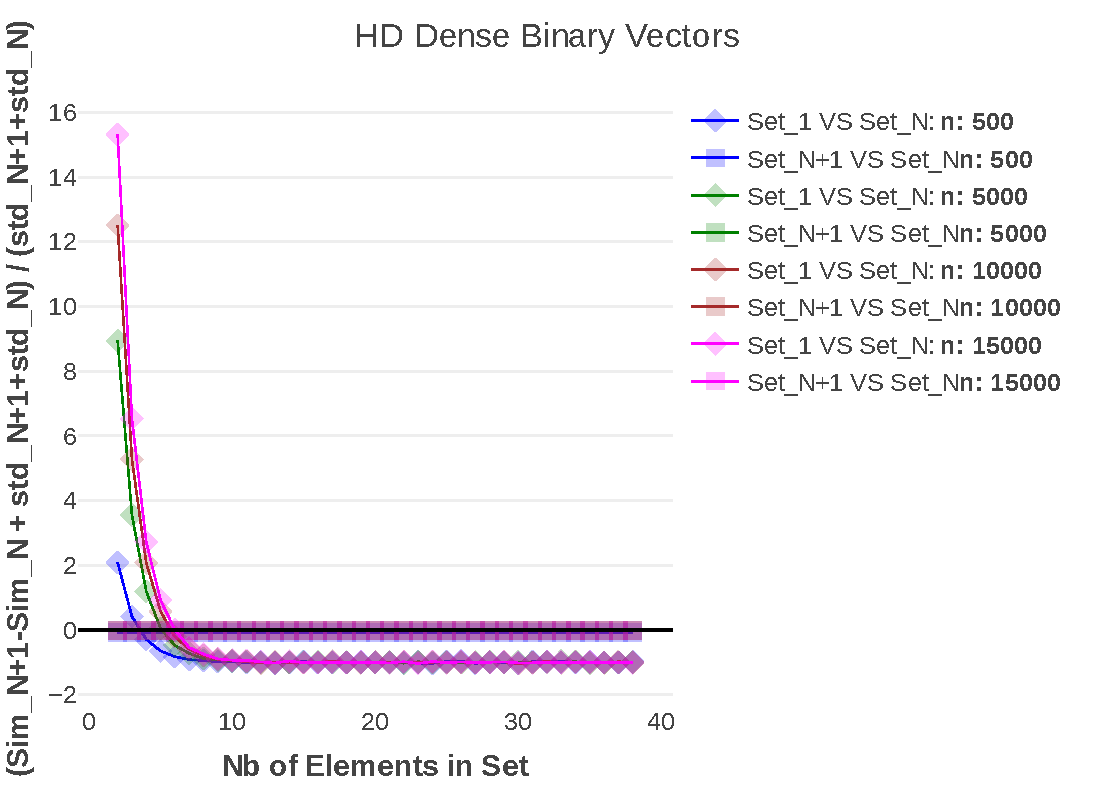
\includegraphics[width=70mm,height=40mm]{../Results/HDBinaryFig1Deltas.pdf} \\
   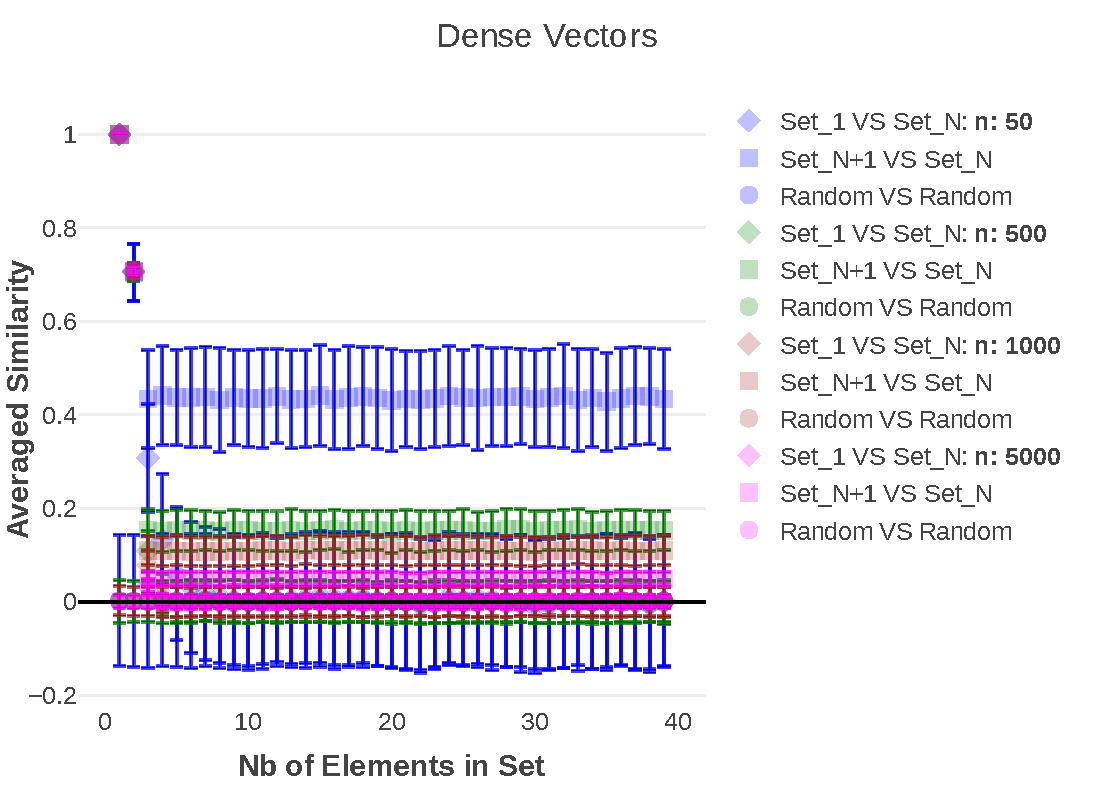
\includegraphics[width=70mm,height=40mm]{../Results/HDDenseFig1Overview.pdf}&
   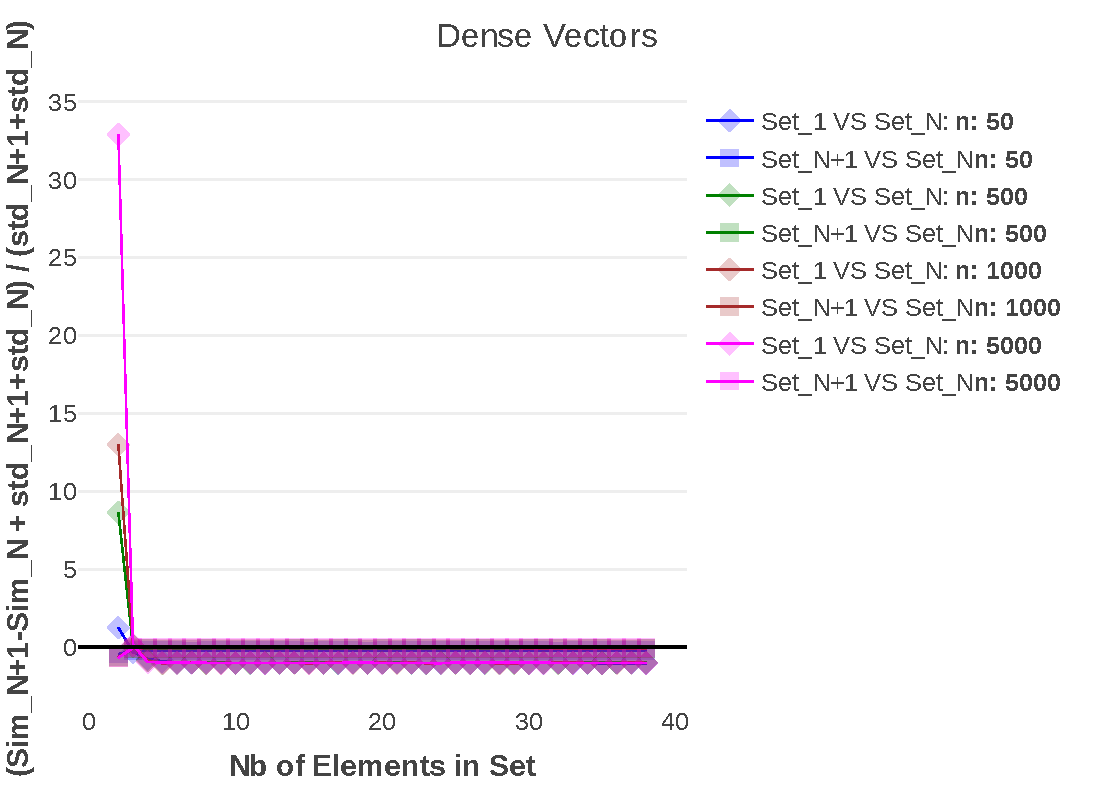
\includegraphics[width=70mm,height=40mm]{../Results/HDDenseFig1Deltas.pdf}
  \end{array}$
 \end{center}
 \caption{After building sets of sizes 1 to N by superposition, one
 		  compares similarities of random elements of same sizes and 			  of sets of sizes $1$ VS $N$, $N$ VS $N+1$ with similar 			  subconstituents. This is done on the left side for sparse 		  and dense binary vectors as well as for dense vectors.
 		  On the right, the relative differences corrected with
 		  the standard deviations are plotted. The y axis is the 
 		  number of standard deviation within which retrieval 
 		  of sub elements would be achievable and being under zero 
 		  indicates incapacity to retrieve data with similarity. 
 		  While dense vectors information collapses under 	
 		  superposition, large SDM would allow to identify subelements 
		  and distinguish correctly the nearest structures, thus 		      confirming the theory. 
 		  }
 \label{pics:composition}
\end{figure}

\section{Memory Requirements}
We here simply review the models memory scaling behaviours:
\begin{itemize}
\item HD vectors: binary vectors of length $L$ would need  $L \times 2$. However, in practice one use sparse framework with the indices
that are Int16, Int32 or Int64. So one needs $L \times 64$ bits.
\item Dense: A dense Vector of length $L$ filled with $Float64$ needs $L \times 64$ bits.
\item SDM's: binary vectors of length $L$ and $W$ non zero elements needs $W \times 2$.
\end{itemize}
The dense vectors space needed is constant for both HD computing and dense vectors. Inversely, it is linear and proportional to the number of elements superposed for Sparse vectors. 
Notice also that for all the example shown in Fig.\ref{pics:composition}, the SDM's have by far the lowest memory requirements.

\section{Discussion and Conclusion}
We have experimented with various 
vector types and sizes, focusing on the superpositions of atomic elements, we have illustrated and confirmed that large sparse vectors are the more robust containers for storing information. We observed that a large number of events could be encoded with minimal space and computational costs.

 As a results, super sparse/superlarge SDM's are very well suited for one shot learning of events combinations storage. 




\begin{thebibliography}{9}

\bibitem{kanerva1}
  P. Kanerva,
  \textit{\LaTeX: Hyperdimensional Computing},
  Addison Wesley, Massachusetts,
  2nd edition,
  1994.
 
%\bibitem{holographic}
%	Tony Plate, 
%	\textit{\LaTeX: Holographic Reduced Representations: Convolution Algebra for Compositional Distributed Representations}

\bibitem{kanerva2}
 \textit{Sparse Distributed Memory}
 Kanerva, Pentti (1988).  The MIT Press. ISBN 978-0-262-11132-4

\end{thebibliography}

\begin{comment}
\pagebreak
\section{Appendix}
\appendix

\section{HD computing}
%Refering to Kanerva's introduction to Hyperdimensional computing ().
\subsection{Kanerva's Hyperdimensional Computer}

We introduce Kanerva brain inspired computing basic vectors are binary containers of 10000 binary elements (or hypervectors) $\{0,\, 1\}$, denoted by Latin letters (A, B, X, ...).
We next introduce the set of all the possible permutations
 on the above vectors, denoted by greek letter ($\Pi, \Gamma, \Lambda, ..$).
 
 The operations considered are thus permutations ($\Pi X$) on hypervectors
 as well as XOR multiplication between them, denoted $\star$ (acting as follows: 
 $0011\dots 10 \quad \mathrm{XOR} \quad 0101\dots 00 = 0110\dots 10$).
 
 Within this setup, Kanerva builds a notion of distance
 $d(A;\, B) = \mid A \star B \mid$ and observes the existence of an identity element $O = 0\dots 0$ with properties $A\star A = O$ and $A\star O = A$.
 Further properties include commutatitivity, invariance of distances under permutation or multiplication by another hypervectors.
 

\subsection{Kanerva's cognitive code}
With the above algebra and exploiting the quasi orthogonality of random hypervectors, Kanerva realises that one could build the following structures: 
\begin{enumerate}
\item Sets are represented with sum of hypervectors (after normalisation), i.e.
$S = A + B + C  $. In practice, $S$ gets normalised with $\|\dots\|_{\#3}$ representing rounding to $\{0,\,1\}$ after division by 3.
\item Records are composed through binding and summation as follows:\\
$R = A \star X + B\star Y$ , where for instance A, X, B, Y could represent 
gender, male, nationality, french respectively or A the dictionary $\{gender: male,  nationality: french\}$. 
\item Sequences are more convenientely modelled with the help of a random permutation $\Pi$: 
$S =A + \Pi B + \Pi \, (\Pi C)$.
\end{enumerate}
Advantages and purpose of the above representations are mainly robustness 
under composition and querying by hypervectors.

For this, the architecture needs a so-called item memory, a dictionary mapping each elements to a unique random hypervector.
 An important point here is that analysis then shows that one could almost surely retrieve each random elements stored in S because for a random hypervector $V$, $d(S;\, A) \gg d(S; \, V)$. On a similar manner, applying with XOR $A$ on $R$ or permuting $\Pi^N$ on $S$ would allow to robustly extract respectively $X$ and the $N$th element of S (using $\Pi^{2} = Identity$). 

The robustness of the architecture described above gradually weakens when the number of elements involved in the above composition increase.
However, they are at the core of the one shot as well as statistical learning strategies in HD computing.
   
\subsection{Cognitive code on sparse vectors}
For SDM's, the above relation still holds and thus one can use the same code. For instance, denoting $Idces(A)$ the integers list of 
indices of the SDM $A$. For $A$ and $B$ SDM's, one has for
$V=A\star B$ the following approximation $Idces(V) \cong Idces(A) + Idces(B)$. Thus, in high dimensions and for classical computing, better computational performances are achieved with sparse frameworks and using simpler permutations, like shifts.

\end{comment}


\end{document}
